\section{\bf Formal languges}

In this section we introduce some basic definitions from the formal language theory, and describe Valiant's parsing algorithm on which we base our solution.

An alphabet $\Sigma$ is a finite nonempty set of symbols.
$\Sigma^{*}$ is a set of all finite strings over $\Sigma$.
A contex-free grammar $G_S$ is a quadruple $(\Sigma, N, R, S)$, where $\Sigma$ is a finite set of terminals, $N$ is a finite set of nonterminals, $R$ is a finite set of productions of the form $A \rightarrow \beta$, where $\Sigma \cap N = \varnothing$, $A \in N, \beta \in V^{*}$, $V = \Sigma \cup N$ and $S \in N$ is a start symbol.
Context-free grammar $G_S = (\Sigma, N, R, S)$ is said to be in Chomsky normal form if all productions in $R$ are of the form: $A \rightarrow BC$, $A \rightarrow a$, or $S \rightarrow \varepsilon$, where $A, B, C \in N, a \in \Sigma, \varepsilon$ is an empty string.
$L_{G}(S) = \{ \omega | S\xrightarrow[G_S]{*} \omega\}$ is a language specified by the grammar $G_{S} = (\Sigma, N, R, S)$, where $A \xrightarrow[G_S]{*} \omega$ means that $\omega$ can be derived in a finite number of rules applications from the start symbol $S$.

\subsection{\bf \it Valiant's parsing algorithm}

Tabular parsing algorithms construct a matrix $T$, cells of which are filled with nonterminals from which the corresponding substring can be derived. 
These algorithms are usually work with the grammar in Chomsky normal form.
For $G_S=(\Sigma, N, R, S)$, $T_{i, j} =  \{ A | A \in N, a_{i + 1} \dots a_{j} \in L_{G}(A)\} \quad \forall i < j$.

The elements of $T$ are filled successively starting with $T_{i - 1, i} = \{ A | A \rightarrow a_{i} \in R\}.$
Then, $T_{i, j} = f(P_{i, j}),$ where
$P_{i, j} = \bigcup\limits_{k = i + 1}^{j - 1} T_{i,k} \times T_{k, j}$ and
$f(P) = \{A | \exists A \rightarrow BC \in R : (B, C) \in P\}.$
Finally, the input string $a_{1}a_{2} \dots a_{n}$ belongs to $L_{G}(S)$ iff $S \in T_{0, n}$.

If all cells are filled sequentially, the time complexity of this algorithm is $O(n^3)$.
Valiant proposed to offload the most intensive computations to the Boolean matrix multiplication. 
As the most time-consuming is computing $\bigcup\limits_{k = i + 1}^{j - 1} T_{i, k} \times T_{k, j}$, Valiant's idea is to compute $T_{i, j}$ by multiplication of submatrices of $T$.
Multiplication of two submatrices of parsing table $T$ is defined as follows.
Let $X \in (2^N)^{m \times l}$ and $Y \in (2^N)^{l \times n}$ be two submatrices of the parsing table $T$. 
Then, $X \times Y = Z$, where $Z \in (2^{N \times N})^{m \times n}$ and $Z_{i, j} = \bigcup\limits_{k = 1}^{l} X_{i, k} \times Y_{k, j}$.

Note that the computation of $X \times Y$  can be replaced by the multiplication of $|N|^2$ Boolean matrices (for each nonterminal pair).
Denote the matrix corresponding to the pair $(B, C) \in N \times N$ as $Z^{(B, C)}$, then $Z_{i, j}^{(B, C)} = 1$ iff $(B, C) \in Z_{i, j}$.
It should also be noted that $Z^{(B, C)} = X^{B} \times Y^{C}$.
Each Boolean matrix multiplication can be computed independently.
Following these changes, time complexity of this algorithm is $O(|G|BMM(n)log(n))$ for an input string of length $n$, where $BMM(n)$ is the number of operations needed to multiply two Boolean matrices of size $n \times n$.

Valiant's algorithm written as proposed by Okhotin is presented in listing~\ref{algo:valiant}.
All elements of $T$ and $P$ are initialized by empty sets.
Then, the elements of these two table are successively filled by two recursive procedures.

% Algorithm1
\begin{algorithm}[h]
\SetAlgoNoLine
\KwIn{Grammar $G = (\Sigma, N, R, S), w = a_{1} \dots a_{n}, n \geq 1, a_{i} \in \Sigma$, where  $n + 1 = 2^k$}
\underline{main()}{:}{

 \textit{compute(0, n + 1)\;}
 accept if and only if $S \in T_{0, n}$
 \linebreak
 }

\underline{compute(\textit{l, m})}{:}{

 \If {$m - l \geq 4$}{
     \textit{compute(l, $\frac{l+m}{2}$)\;
     compute($\frac{l+m}{2}$, m)}}
 \textit{complete(l, $\frac{l+m}{2}$, $\frac{l+m}{2}$, m)}
 \linebreak
 }

\underline{complete(\textit{l, m}, $l^\prime$, $m^\prime$)}{:}{

 \lIf {$m - l = 4$ and $m = l^\prime$}{$T_{l, l + 1} = \{A | A \rightarrow a_{l+ 1} \in R\}$}
 \lElseIf{$m - l = 1$ and $m < l^\prime$}{ $T_{l, l'} = f(P_{l, l'})$}
 \ElseIf{$m - l > 1$}{
    $\textit{leftgrounded} = (l, \frac{l+m}{2}, \frac{l+m}{2}, m), \textit{rightgrounded} = (l', \frac{l'+m'}{2}, \frac{l'+m'}{2}, m')$,

    $\textit{bottom} = (\frac{l+m}{2}, m, l', \frac{l'+m'}{2}), left = (l, \frac{l+m}{2}, l', \frac{l'+m'}{2})$,

    $\textit{right} = (\frac{l+m}{2}, m, \frac{l'+m'}{2}, m'), top = (l, \frac{l+m}{2}, \frac{l'+m'}{2}, m')$\;
    \textit{complete(bottom)}\;
    $P_{\textit{left}} = P_{\textit{left}} \cup (T_{\textit{leftgrounded}} \times T_{\textit{bottom}})$\;
    \textit{complete(left)}\;
    $P_{\textit{right}} = P_{\textit{right}} \cup (T_{\textit{bottom}} \times T_{\textit{rightgrounded}})$\;
    \textit{complete(right)}\;
    $P_{\textit{top}} = P_{\textit{top}} \cup (T_{\textit{leftgrounded}} \times T_{\textit{right}})$\;
    $P_{\textit{top}} = P_{\textit{top}} \cup (T_{\textit{left}} \times T_{\textit{rightgrounded}})$\;
    \textit{complete(top)}
    }
 }
\caption{Parsing by Matrix Multiplication: Valiant's Version}
\label{algo:valiant}
\end{algorithm}

The procedure $compute(l, m)$ computes correct values of $T_{i,j}$ for all $l \le i < j < m$.

The procedure $complete(l, m, l', m')$ constructs the submatrix $T_{i, j}$ for all $l \le i < m$, $l' \le j < m'$. This procedure assumes $T_{i, j}$ for all $l \leq i < j < m,  l' \leq i < j < m'$ are already constructed and the current value of  $P[i, j] =  \{ (B, C) |\exists k, (m \le k < l'), a_{i + 1} \dots a_{k} \in L(B), a_{k + 1} \dots a_{j} \in L(C)\}$ for all $l \leq i < m,  l' \leq j < m'$.
The submatrix partition during the procedure call is shown in figure~\ref{fig2}.


\begin{figure}
\vspace{3mm}
 \begin{center}
    \begin{minipage}{0.48\textwidth}
        \centering
        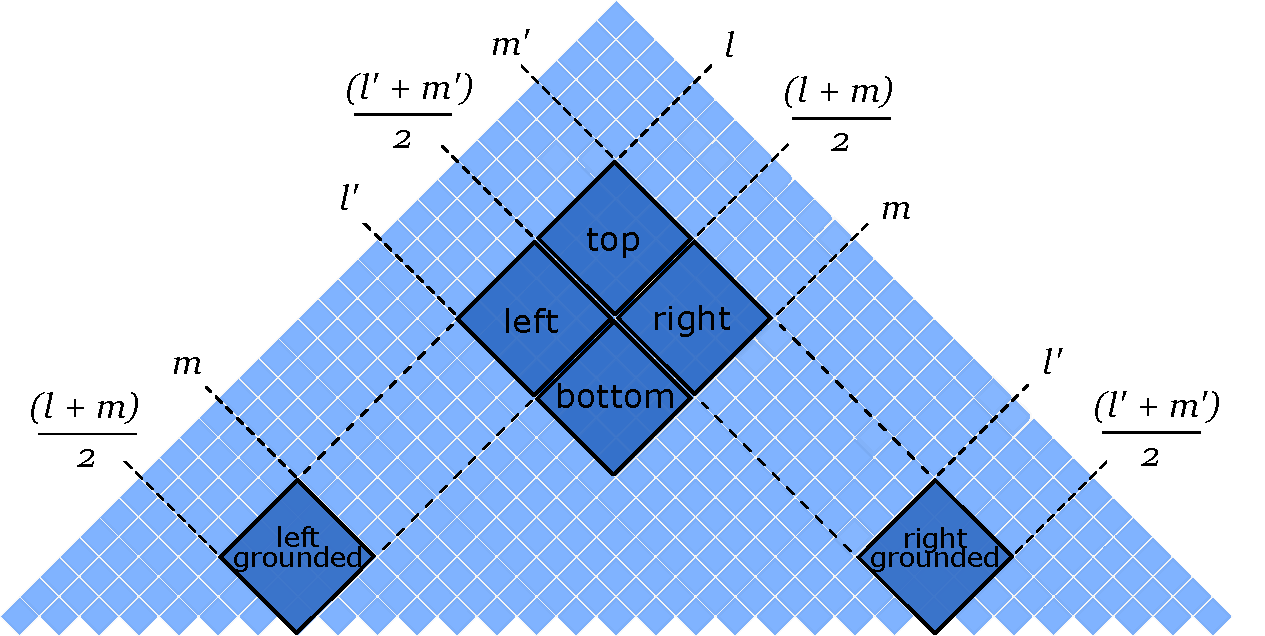
\includegraphics[width=6cm]{pictures/splitting_with_grounded.pdf}
        \caption{Matrix partition used in procedure \textit{complete(l, m, l', m')}}
        \label{fig1}
    \end{minipage}\hfill
    \begin{minipage}{0.48\textwidth}
        \centering
        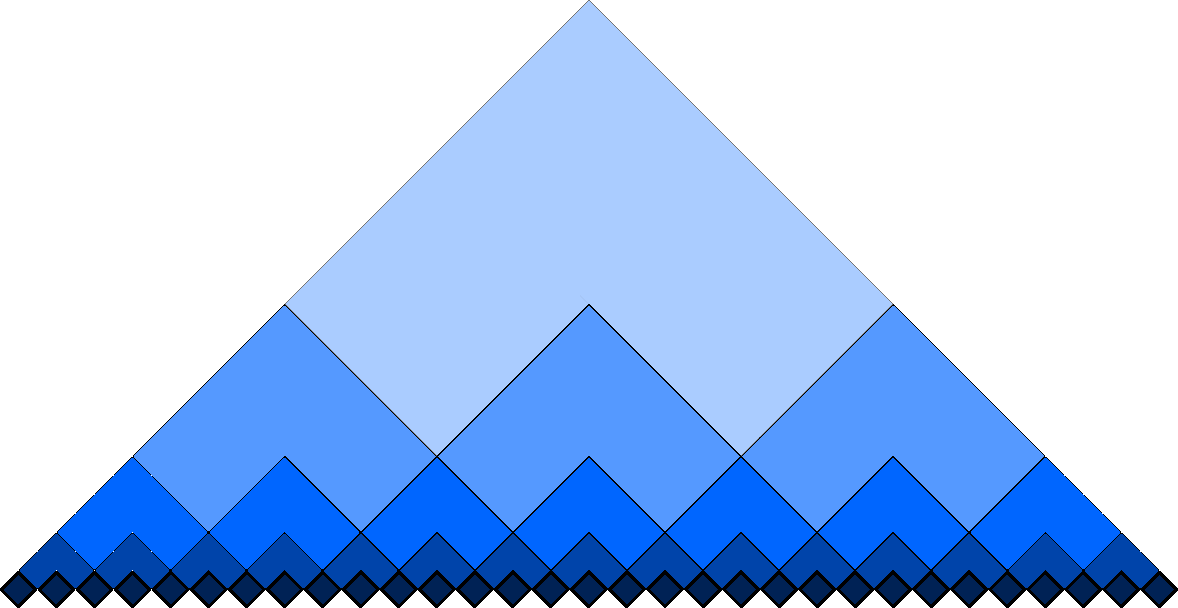
\includegraphics[width=6cm]{pictures/layers.pdf}
        \caption{Matrix partition on V-shaped layers used in modification}
        \label{fig2}
    \end{minipage}
 \end{center}
\vspace{-8mm}
\end{figure}

A simple example of parsing with the Valiant's algorithm is presented in figure~\ref{fig3}.
Only several steps are shown, but it is enough to compare our version with the original algorithm.

\begin{figure}
\vspace{3mm}
 \begin{center}
 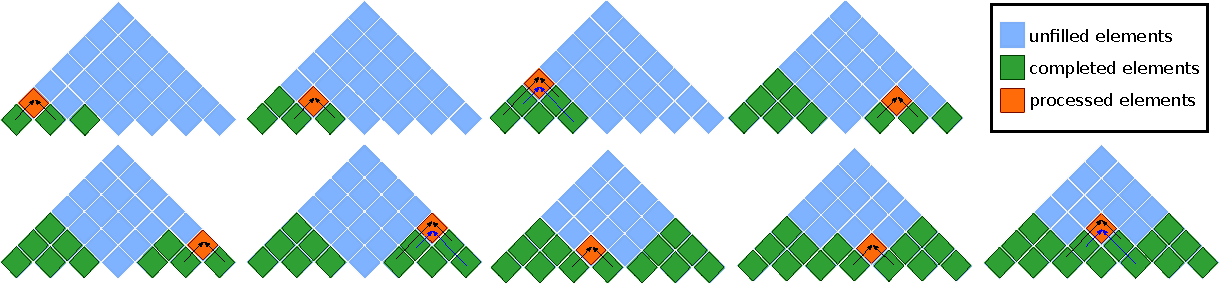
\includegraphics[width=12cm]{pictures/valbeg2.pdf}
    \caption{An example of beginning of Valiant's algorithm}
    \label{fig3}
\end{center}
\vspace{-8mm}
\end{figure}